% !TeX root = ./main.tex
\documentclass[main]{subfiles}
\begin{document}

\chapter{Расширения полей}


\begin{definition}
    Говорят, что задано расширение поля $L / K$ (читается $L$ над $K$),
     если задано поле $L$ и подполе $K$.
\end{definition}

\begin{example}
    \begin{enumerate}
        \item $\C / \R$
        \item $ \R / \Q $
        \item  $ K / K$ для любого $K$
        \item  $K(X) / K $ для любого $K$
    \end{enumerate}
  
\end{example}

Если $L / K$ -- расширение, то $L$ можно рассматривать как линейное пространство над $K$.
$L / K$ называется конечным расширением, если $\dim_k L < \infty$. 
$[L:K] = \dim_k L $ -- степень расширения $L / K$. В противном случае
$L / K$ называются бесконечным.

\begin{example}
    \begin{enumerate}
        \item $[\C:\R] = 2$
        \item $[\R : \Q ] = \infty$
        \item  $ [K:K] = 1$
        \item $[K(X):K]= \infty $ 
    \end{enumerate}
\end{example}

\begin{proposition}
    Пусть $L / K, M / K$ -- конечные расширения. Тогда $M / K$ -- тоже
    конечное расширение и $[M:K] = [M:L] \cdot [L:K]$.
    $M / L / K $ -- башня полей.
\end{proposition}

\begin{proof}
    Пусть $e_1, \ldots , e_l $ -- базис $L$ как линейного пространстнства $/ K$.
    $f_1, \ldots , f_n$ -- базис $M$ как линейного пространства $/ L$. Проверим 
    $(e_i f_j \ | \ 1 \leq i \leq l, 1 \leq j \leq m)$ -- базис $M / K$. Пусть $c \in M
    \Rightarrow c = b_1f_1 + \ldots + b_mf_m, \ b_1, \ldots, b_m \in L \Rightarrow 
        c = (a_{11}e_1 + \ldots + a_{1l}e_l)f_1 + \ldots + (a_{m1}e_1 + \ldots + a_{ml}e_l)f_m = \\
        = \sum^n_{i=1} \sum^l_{j=1} a_{ij}e_jf_i, \ a_{ij} \in K 
        \Rightarrow Lin(e_jf_i \ | \ 1 \leq j \leq l, 1 \leq i \leq m) = M$.

        Пусть $\sum_{i,j} a_{ij} e_if_j = 0 $.
         $\sum_{j} \left( \underbrace{\sum_{i} a_{ij} e_i}_{\in L} \right) f_j, \ f_1, \ldots, f_m \text{ -- базис } M / L 
         \Rightarrow \sum_i a_{ij}  e_i = 0, \ j = 1, \ldots, m, \ e_1, \ldots, e_l$ -- базис $L / K
         \Rightarrow$ все $a_{ij} = 0$.
   
\end{proof}

\begin{definition}[Алгебраический элемент]
    Пусть $L / K$ -- расширение, $a \in L$. $a$ называется алгебраическим
    над $K$, если существует $f \in K[X], \ f \ne 0$, такой что $f(a) = 0 $. В противном случае, $a$
    называется трансцендентным $/ K$.
\end{definition}

\begin{example}
    $\sqrt{2}$ алгебраичен над $\mathbb{Q}, \ f = X^2-2$
\end{example}

$L / K$ называется алгебраическим, если все его элементы алгебраичны $/ K$.
В противном случае, $L / K$ называется трансцендентным.

\begin{example}
    \begin{enumerate}
        \item $ \C / \R $ -- алгебраическое.
        \item $\R / \Q$ -- трансцендентное, например, $\pi$ -- трансцендентное $/ Q$.
        Таким образом, алгебраические числа (в $\R$) образуют счётное множество.
        \item  $K(X) / K$ -- трансцендентное,  $X$ -- трансцендентный, $f(X) = \frac{f(X)}{1}$.
    \end{enumerate}
\end{example}


\begin{proposition}
    Любое конечное расширение поля -- алгебраично.
\end{proposition}

\begin{proof}
    Пусть $[L:K] = d$.
    \begin{gather*}
        a \in L, \d \underbrace{1, a, a^2, \ldots, a_d}_{d+1} \\
        \Rightarrow \exists h_0, h_1, \ldots, h_d \in K : b_0 + b_1a + \ldots b_da^d = 0 \text{ и не все } b_i = 0\\
        f:= b_dX^d + \ldots b_1 X + b_0 \ne 0 \\
        f(a) = 0 \Rightarrow a \text{ -- алгебраическое }
    \end{gather*}
\end{proof}

\begin{proposition}
    Пусть $L / K$, $a \in L$ -- алгебрическое. Тогда $ \{ f \in K[X] \ | \  f(a) = 0 \} = (p), \ 
    p$ -- неприводимый многочлен из $K[X]$.
\end{proposition}

\begin{proof}
    $ I = \{ f \in K[X] | f(x) \ 0 \} \text{ -- подгруппа в } K[X]$.

    \[\left.
    \begin{gathered}
        f \in I \\
        g \in K[X]
    \end{gathered} \right. \Rightarrow (gf)(a) = g(a)\underbrace{f(a)}_{0} = 0 \Rightarrow gf \in I \]

    Таким образом, $I$ -- идеал $\Rightarrow I = (p)$ в $K[X]$. 

    Проверим, что $p$ -- неприводимый.
  
    \[p = fg, \ 
    p(a) = 0 \Rightarrow f(a)g(a) = 0 \Rightarrow \left[ \begin{gathered}
        f(a) > 0 \\
        g(a) > 0
    \end{gathered} \right. \]
    \[ \Rightarrow \left[ \begin{gathered}
        f \in I = (p) \\
        g \in I = (p)
    \end{gathered} \right. \Rightarrow \left[ \begin{gathered}
        f \sim p \\
        g \sim p
    \end{gathered} \right. \]
\end{proof}
Такой многочлен $p$ будем обозначать $Irr_K a$. Например $Irr_{\R} i = x^2 + 1$. \\

\begin{definition}
    Пусть $L / K : \quad a_1, \ldots, a_m \in L$. 
    $K(a_1, \ldots, a_m) := \bigcap_{\underset{a_1, \ldots, a_m \in F}{\underset{K \subset F}{F \text{ подполе } L}}}
    \text{ -- подполе } L$.
    Назовем его расширением $K$, порожденным $a_1, \ldots, a_m$.
\end{definition}

\begin{definition}
    Пусть $L / K$ -- расширение, если $\exists \ a_1, \ldots, a_m \in L$, т.ч.
    $K(a_1, \ldots, a_m) = L$, то $L / K $ называется конечно порожденным.
\end{definition}

\begin{proposition}
    Пусть $L / K$ -- конечное  расширение, тогда $L / K$ конечно порожденное.
\end{proposition}

\begin{proof}
    $e_1, \ldots , e_n$ -- базис $L/K$. $a_1e_1 + \ldots + a_ne_n \in  K(e_1, \ldots, e_n)  \Rightarrow K(e_1, \ldots, e_n) = L$.
\end{proof}

\begin{remark}
    Обратное неверно. $K(X) / K$ -- порождается одним элементом $(x)$, но не конечное, так как трансцендентное.
\end{remark}

\begin{definition}[Простое расширение]
    $L / K$ называется простым, если $\exists \ a \in L$, т.ч. $L = K(a)$.
\end{definition}

\begin{proposition}
    Пусть $L / K$ -- простое алгебраическое расширение, то есть $L = K(a), \ a$ -- алгебраический над $K$.
    Тогда $L \cong K[X] / (p)$, где $p = Irr_K a$.
\end{proposition}

\begin{proof}
    \[ \underset{f \mapsto f(a)}{K[X] \stackrel{\alpha}{\longrightarrow}} L \]
    \[ \Ker \alpha = (p) \] 
    \[  \left. \begin{gathered}
        \Rightarrow \Im \alpha \cong K[X] / (p), p \text{ -- неприводимый} \Rightarrow \Im \alpha \text{ -- поле } \\
        K \subset \Im \alpha \text{, т.к. } \alpha(c) = c \ (c = const) \\
        a \in \Im \alpha \text{ т.к. } \alpha(x) = a
    \end{gathered} \right) \Rightarrow \]
    \[\Rightarrow K(a) \subset \Im \alpha = L \]
    
   Таким образом, $L \cong K(X)  / (p)$.
\end{proof}

\marginpar{30.11.22}

\begin{corollary}
    \begin{enumerate}
        \item Если $F$ -- минимальный многочлен $a$, $deg f = d$, то $[K(a):K] = d$, и базисом $K(a)$, как линейного пространства над $K$, служит
    семейство $1, a, a^2, \ldots, a^{d-1}$.
        \item Если есть еще одно расширение $K(b)/K$, и минимальный многочлен $b$ также $f$, то существует изоморфизм
        $\underset{\sum_{i=0}^{d-1}\alpha_ia^i \mapsto \sum_{i=0}^{d-1}\alpha_ib^i}{K(a) \rightarrow K(b)} (\alpha_i \in K)$.
    \end{enumerate}
\end{corollary}

\begin{proof}
    \begin{enumerate}
    \item Есть изоморфизм $K[X]/(f) \underset{\rightarrow}{\sim } K(a)$ -- изоморфизм полей и линейных пространств $/K$. Рассмотрим первое пространство: 
    $K[X]/(f) = \{\overline{\alpha_0 + \alpha_1X + \ldots + \alpha_{d-1}X^{d-1}} \ | \ \alpha_0, \ldots, \alpha_{d-1} \in K\} = 
    \{\alpha_0\overline{1} + \alpha_1\overline{X} + \ldots + \alpha_{d-1}\overline{X^{d-1}} \ | \ \alpha_0, \ldots, \alpha_{d-1} \in K\}$.
    Очевидно, $\overline{1}, \overline{X}, \ldots, \overline{X^{d-1}}$ -- линейно независимые
    ($\alpha_0 + \alpha_1X + \ldots + \alpha_{d-1}X^{d-1} \ne\equiv 0 \mod f$). Таким образом, 
    $\overline{1}, \overline{X}, \ldots, \overline{X^{d-1}}$ -- базис $K[X]/(f)$ 
    $\Rightarrow 1, a, a^2, \ldots, a^{d-1}$ -- базис $K(a)$.
    \item 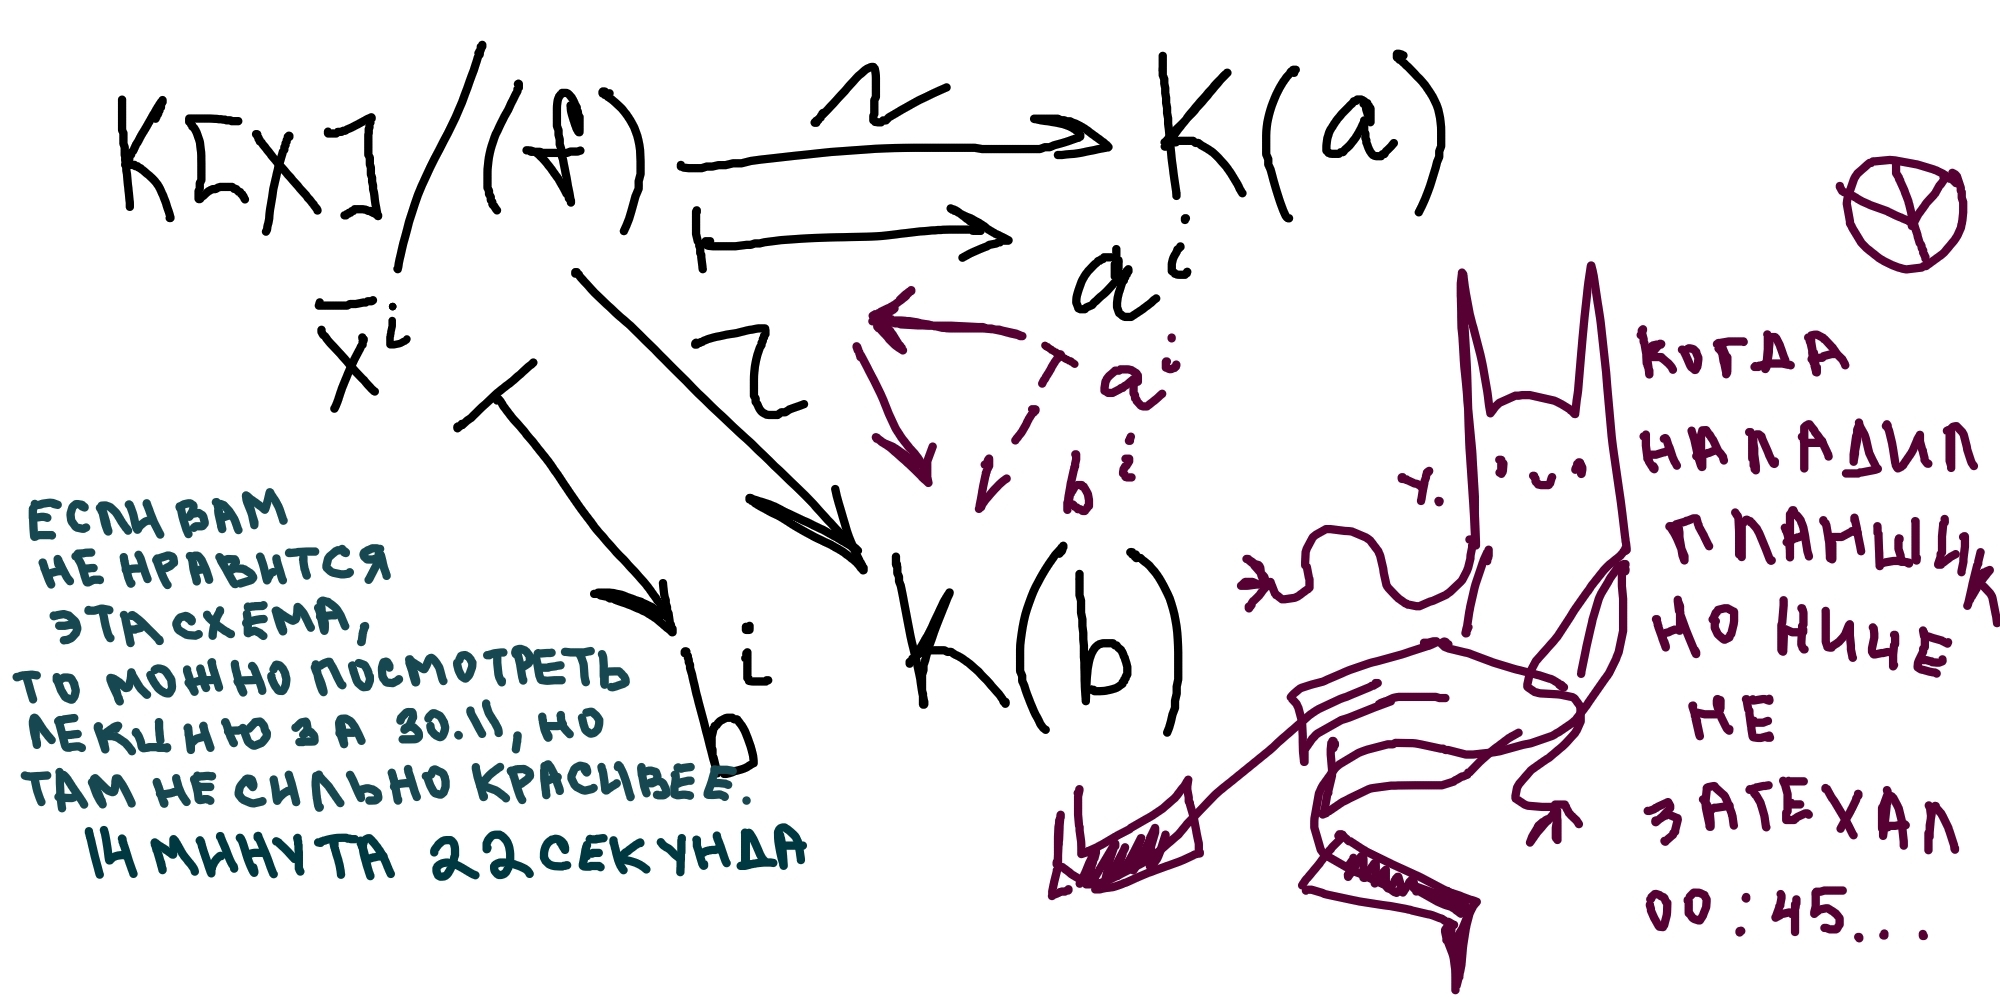
\includegraphics[width=0.8\textwidth]{ugly_scheme.jpg}
    \end{enumerate}
\end{proof}

\begin{proposition}
    Пусть $f \in K[X]$ -- неприводимый. Тогда существует расширение $K(a)/K$, такое что $Irr_K(a) = f$.
\end{proposition}

\begin{proof}
    $L = K[X] / (f)$ -- поле, так как $f$ неприводим. $\underset{c \mapsto \overline{c}}{K \hookrightarrow L}$ отожествляет $c$ с $\overline{c}$. 
    Очевидно, $L = K(\underbrace{\overline{X}}_{a:=})$, любой элемент этого поля представим в виде $\overline{\sum \alpha_i x^i} = \sum \overline{\alpha_i} \overline{X^i} =
    \sum \alpha_i \overline{X^i}$. $Irr_K X = f$, так как $f(\overline{x}) = \overline{F} = 0$ и $f$ неприводим.
\end{proof}

%уже здесь почему-то не собиралось

\begin{proposition}
    Пусть $a$ трансцендентен над $K$. Тогда $K(a) \cong K(X)$.
\end{proposition}

\begin{proof}
    \begin{gather*}
        \underset{\underbrace{\frac{f}{g}}_{g \neq 0} \mapsto \underbrace{\frac{f(a)}{g(a)}}_{g(a) \neq 0 \text{, т.к. } a \text{ тр.}}}{K(X) \xrightarrow{\mse} K(a)} \\
        \Im \mse \text{ -- подполе в } К(a) \\
        K \subset \Im \mse \ (c = \mse(c)) \\
        a \in \Im \mse \ (a = \mse(X)) \\
        \Rightarrow \Im \mse = K(a)
    \end{gather*}
\end{proof} 

\begin{example}
    Пусть $K = \F_2, \ f = x^2 + x + 1, \ L = \F_2(a)$, где $a$ -- корень $f$. 
    Составим таблицы сложения и умножения: 
    \begin{gather*}
        \begin{array}{c|c|c|c|c}
            + & 0 & 1 & a & 1 + a \\ \hline
            0 & 0 & 1 & a & 1 + a \\ \hline
            1 & 1 & 0 & 1+a & a \\ \hline
            a & a & 1 + a & 0 & 1 \\ \hline
            1 + a & 1 + a & a & 1 & 0 
        \end{array} \quad
        \begin{array}{c|c|c|c|c}
            \cdot & 0 & 1 & a & 1 + a \\ \hline
            0 & 0 & 0 & 0 & 0 \\ \hline
            1 & 0 & 1 & a & 1+a \\ \hline
            a & 0 & a & 1 + a & 1 \\ \hline
            1 + a & 0 & 1 + a & 1 & a 
        \end{array}
    \end{gather*}
\end{example}

\begin{definition}
    Расширение $L$ поля $K$ называется полем разложения многочлена $f \in K[X]$, если:
    \begin{enumerate}
        \item В $L[X] \ f$ раскладывается на линейные множители.
        \item $L = K(a_1, \ldots, a_m), \ a_1, \ldots, a_m$ -- все корни $f$ в $L$.
    \end{enumerate}
\end{definition}

\begin{example}
    \begin{enumerate}
        \item $\C/\R$ -- поле разложения $X^2 + 1$.
        \item $K = \Q(\sqrt[4]{2})$ -- не поле разложения $X^4-2$ над $\Q$.
        В $K[X] \ X^4 - 2 = (X - \sqrt[4]{2})(X + \sqrt[4]{2})(X^2 + \sqrt{2})$.
        \item $K' = \Q(\sqrt[4]{2}, i\sqrt[4]{2}) = \Q(\sqrt[4]{2}, i)$ -- поле разложения $X^4 - 2$ над $\Q$. 
    \end{enumerate}
\end{example}

\begin{proposition}
    Пусть $K$ поле, $f \in K[X]$. Тогда у $f$ существует поле разложения над $K$.
\end{proposition}

\begin{proof}
    Индукция по  $d = deg f$.

 $d \leq 1$: $K$ -- поле разложения $f$.

 $d > 1$: $p$ -- неприводимый делитель $f$. $L = K(a), \ p(a) = 0$. $f(a) = 0 \xRightarrow{\text{т. Безу}} f = (X - a)g$.
 $g \in L[X], \ deg g = d-1$.

 По индукционному предположению существует $M/L$ -- поле разложения $g$. В $M[X] \ g = c(X - a_1)\ldots(X - a_{d-1}) \Rightarrow
 f = c(x - a)(x - a_1)\ldots(x - a_{d-1}).\ M = L(a_1, \ldots, a_{d-1}) = K(a)(a_1, \ldots, a_{d-1}) = K(a, a_1, \ldots, a_{d-1})$.
\end{proof}

Изоморфизмом между расширениями $L_1/K$ и $L_2/K$ -- это изоморфизм $\sigma$: $L_1 \backsimeq L_2$ такой, что $\forall \ a \in K: \ \sigma(a) = a$.
 
\begin{proposition}
    $L/K$ -- расширение. Тогда 2 условия эквивалентны:
    \begin{enumerate}
        \item $L/K$ конечно.
        \item $L = K(a_1, \ldots, a_n), \ a_1, \ldots, a_n$ -- алгебраические над $K$.
    \end{enumerate}
\end{proposition}

\begin{proof}
    1 $\Rightarrow$ 2: Пусть $\theta_1, \ldots, \theta_n$ -- алгебраичсекие над $K \Rightarrow
    K(\theta_1, \ldots, \theta_n) = L$, все элементы $L$ алгебраичны над $K$.

    2 $\Rightarrow$ 1: Индукция по $n$. $n = 0 \Rightarrow L = K$.
    $n > 0 \Rightarrow L = K'(a_n), \ K' = K(a_1, \ldots, a_{n-1}),
    [K':K] < \infty$ по ИП, $[L:K'] = d, \ d = deg Irr_{K'}a_n < \infty, 
    [L:K] = [L:K'][K':K] < \infty$.
\end{proof}

\begin{corollary}
    Пусть $a, \ b$  -- алгебраичны над $K$. Тогда $a + b, \ ab$ -- алгебраичны над $K$. 
\end{corollary}
    
\begin{proof}
    $a, \ b$  -- алгебраичны над $K \Rightarrow K(a, b)/K$ -- конечное $\Rightarrow$ алгебраическое.
    $a+b, \ ab \in K(a, b) \Rightarrow a+b, \ ab$ -- алгебраичны над $K$.
\end{proof}
\end{document}